%% beamerthemeImperialPoster v1.0 2016/10/01
%% Beamer poster theme created for Imperial College by LianTze Lim (Overleaf)
%% LICENSE: LPPL 1.3
%%
%% This is the example poster demonstrating use
%% of the Imperial College Beamer Poster Theme
\documentclass[xcolor={table}]{beamer}
%% Possible paper sizes: a0, a0b, a1, a2, a3, a4 (although Imperial College posters are usually A0 or A1).
%% Possible orientations: portrait, landscape
%% Font sizes can be changed using the scale option.
\usepackage[size=a0,orientation=portrait,scale=1.55]{beamerposter}
\usepackage{amsmath} 						% Adds mathematical features for equations
\DeclareMathOperator{\Tr}{Tr}				% This is adding in a Trace definition for matrices
\usepackage{bbold}							% Adding in fancy letters for 1 operators etc.
\usepackage{mathtools}						% Adds in text for above/below arrows
\usepackage{physics} 						% Just for absolute values etc.
\usepackage{amssymb}						% For natural numbers symbol
\usepackage{dsfont}                         % for identity double stroke
\usepackage{wrapfig}
\renewcommand{\vec}{\vectorbold}            % if we want to redefine the vector 

\newcommand*{\field}[1]{\mathbb{#1}}%		% Defining the natural numbers
\newcommand*\dif{\mathop{}\!\mathrm{d}}		% Adding additional command for nice looking integration variables dx etc, use like " \dif variable " in integrals 
\newcommand*\bigO{\mathop{}\!\mathcal{O}}   % big O notation
\newcommand\ddfrac[2]{\frac{\displaystyle #1}{\displaystyle #2}}    % for creating bigger fractions that look nicer 

\definecolor{GraphRed}{HTML}{ec1c24}
\definecolor{GraphBlue}{HTML}{00a8f3}
\definecolor{GraphGreen}{HTML}{a1ecb6}
\definecolor{BackgroundBlue}{HTML}{d3e4f0}


\graphicspath{ {images/} }	

\usetheme{ImperialPoster}

%% Four available colour themes
\usecolortheme{ImperialWhite} % Default
% \usecolortheme{ImperialLightBlue}
% \usecolortheme{ImperialDarkBlue}
% \usecolortheme{ImperialBlack}

 
\title{\Huge Condensed Matter Theory}

% \setbeamertemplate{bibliography item}{\insertbiblabel}
% \addbibresource{supersolid.bib}

\begin{document}
\small
\begin{frame}[fragile=singleslide,t]\centering

\maketitle

\begin{tcolorbox}[colback=BackgroundBlue,colframe=ICDeepBlue,fontupper=\color{ICDeepBlue}]
\normalsize
    Condensed matter physics is the study of the immense variety of solids and
    liquids provided by nature or made by humans. Metals, magnets, ceramics,
    semiconductors, foams, membranes, superfluids, superconductors, granular
    systems, polymers, complex liquids, planetary interiors, and graphene are
    examples of the sorts of things we work on.
    Solids and liquids are understood to the extent that the Schrödinger equation
    provides an accurate “grand unified theory” at the atomic scale. However,
    assemblies of huge numbers of simple objects often show emergent behaviour that
    could never have been guessed from their individual properties. One atom on its
    own is a dull thing, but the emergent properties of huge numbers of atoms give
    the world, and our subject, their astonishing variety and richness. The idea of
    emergence is not restricted to atoms. Our Complexity and Networks Group studies
    emergence in social and biological systems.
    Understanding materials also enables us to develop new ones to perform according
    to our wish. Our group has world-leading expertise in 'condensed matter optics'.
    Using nano-photonics and plasmonics, we design 'metamaterials' to manipulate and
    harvest light with unprecedented control.

\end{tcolorbox}

\begin{columns}[onlytextwidth,T]

%%%% First Column
\begin{column}{.47\textwidth}

\begin{block}{Metamaterials}
Imperial is the home of Metamaterials. John Pendry's revolutionary ideas are
simple but change and expand our understanding of the world in profound ways.
Metamaterials exploit the idea that physically structuring on a scale less than
the wavelength can dramatically alter a material’s property. Using man-made
metamaterials, one can construct a perfect lens that, unlike a conventional
lens, does not have limitations in the sharpness of the image or one can guide
light around an object, rendering it in effect invisible, see Fig. 1. Devices
using metamaterials are already finding their way into production and are likely
to become common in the future.
\end{block}

\begin{figure}
    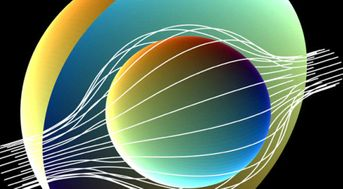
\includegraphics[width=\columnwidth, height=0.15\textheight]{metamaterials.jpg}
    \caption{\footnotesize John Pendry et al. proposed a way to guide light over or around an object using metamaterials with exotic optical properties. The invisibility cloak deflects microwave beams as they flow around an object hidden inside it, in the same way that water in a river flows around a stick.}
\end{figure}

\begin{block}{Complexity Science}
The richness and complexity in condensed matter physics reflects the fact that
new organised behaviour emerges from the collective behaviour of simple
interacting objects, whether they are electrons in a metal or agents in a social
network. The study of emergent phenomena is a central theme of modern condensed
matter physics. We are part of the Centre for Complexity Science at Imperial
which focus on developing and applying transferable tools and techniques to real
world systems in many different contexts: geology (earthquake \& reservoir
engineering), atmospheric physics (rain), biology (evolution \& social insects),
sociology (organisational science), medicine (brain \& heart) and fire safety
(smouldering).
\end{block}

\begin{figure}
    \centering
    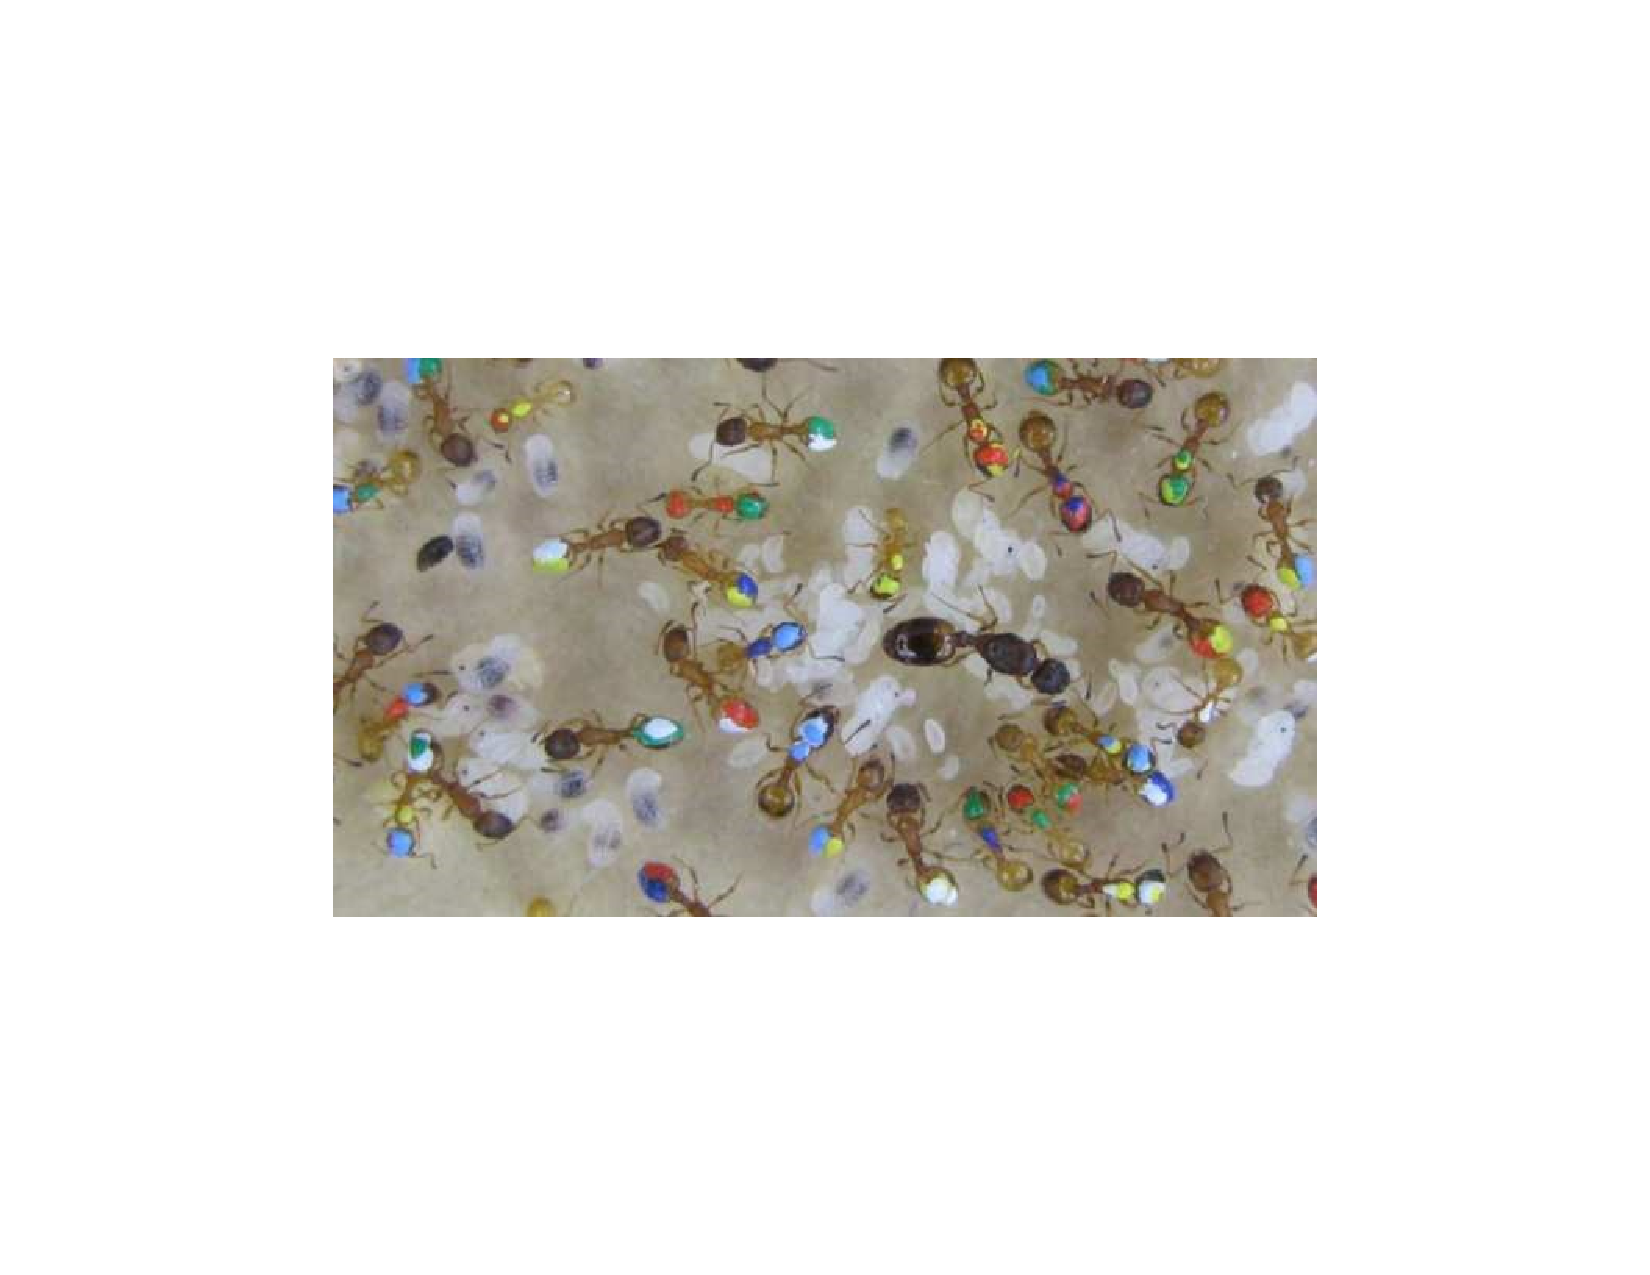
\includegraphics[width=1.\columnwidth, height=0.2\textheight]{AntColony.pdf}
    \caption{\footnotesize An ant-colony is the prime example of a complex system in Nature. The colony is a self-organized adaptive society who’s macroscopic (colony-level) properties originate from interactions at the microscopic level among the individual ants themselves and between individuals and the environment. Without a blue-print, the self-organizing bottom-up structure can accomplish incredible feats that are impossible to complete for ants in isolation.}
\end{figure}

\end{column}

%%%% Second Column
\begin{column}{.47\textwidth}

\begin{block}{Correlated Quantum Systems}
On the microscopic scale, strongly correlated quantum systems exhibit emergent
phenomena in terms of exotic quantum phases of matter in equilibrium or novel
dynamical behaviour out of equilibrium. This can lead to systems exhibiting
novel exchange statistics which allow for quantum computing, to materials that
have additional speeds of sound with a rich and complex set of dynamics, or to
materials which exhibit chirality in the presence of disorder. Our work
encompasses a wide variety of quantum mechanical systems such as
nano-electromechanical devices, liquid helium films and ultracold atomic clouds.
\end{block}

\begin{figure}
    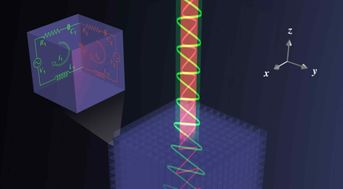
\includegraphics[width=1\columnwidth, height=0.2\textheight]{correlated.jpg}
    \caption{\footnotesize Please insert caption here about relevant image}
\end{figure}

\begin{block}{Physics of Materials}
New materials have played a central role in the development of civilisation from
the Bronze Age to the Semiconductor Age. We have developed widely used
computational codes to solve the equations of quantum mechanics to predict the
electronic behaviour at the nanoscale, structural properties at the microscale,
or material behaviour on macroscopic length and time scales.
\end{block}

\begin{figure}
    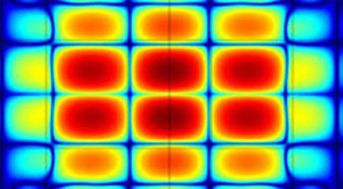
\includegraphics[width=\columnwidth, height=0.2\textheight]{simulation_materials.jpg}
    \caption{\footnotesize Please insert caption here about relevant image}
\end{figure}

\end{column}
\end{columns}

\begin{tcolorbox}[colback=BackgroundBlue,colframe=ICDeepBlue,fontupper=\color{ICDeepBlue}]
    For a showcase of particular projects within each of the 4 areas of
    condensed matter theory, please see the posters in the hall of the Blackett
    Laboratory on Level 8
\end{tcolorbox}

\end{frame}
\end{document}